\chapter{基于互信息正则的分类模型}\label{chap:model}

\section{引言}
在原始的生成对抗网络中,生成器通过将噪声映射成数据,然后由对抗损失函数驱动,进而能够在训练过程中慢慢学习到真实数据的分布信息,最终生成较为逼真的虚假数据。生成对抗网络的特殊性在于它创新性地结合了生成式模型和判别式模型。它在训练生成式模型的同时,也训练了一个判别式模型。其最大贡献在于提出了一个对抗训练的机制,而且本身没有过多的约束,这为后续的研究提供了巨大的可扩展性。\citet{goodfellow2014generative}给出生成对抗网络的模型以及结果之后,在文章最后关于GAN的扩展工作也给出了几点建议:
\begin{enumerate}
  \item 可以为生成器和判别器添加条件信息,此时生成器可以学习到对应的条件分布;
  \item 通过增加一个辅助网络来估计$p(\bd{z}|\bd{x})$,可以进行进一步的统计推断;
  \item 半监督学习:当拥有少量标签信息时,判别器学到特征可以用于提高分类器的性能。
\end{enumerate}

鉴于生成对抗网络具有如此良好的可扩展性,越来越多的学者开始研究该模型\citep{mirza2014conditional,radford2015unsupervised,chongxuan2017triple}。尽管如此,关于生成器如何将噪声映射成数据的细节仍有待探索。许多研究表明,通过对隐变量连续插值,会在生成的图片上得到连续平滑的变化\citep{radford2015unsupervised,chen2016infogan,dumoulin2016adversarially,miyato2018cgans}。然而,大多数变化无法解释并且没有明确的意义。\citet{chen2016infogan}提出的InfoGAN模型将隐变量分解,通过在训练过程中增加隐变量和生成数据之间的互信息,达到了将特征解耦的效果。该模型的隐变量可以明确对应到一个个有意义的数据特征(如MNIST中手写数字的角度、笔画粗细等)。这证明了互信息约束在生成对抗网络中有值得探究的作用。

\section{C-InfoGAN}\label{sec:c-infogan}
%InfoCatGAN无法同时获得较高的准确率和生成质量,只能通过正则系数$\lambda_1$实现二者的性能折中。考虑到InfoGAN模型中的隐变量可以较好地绑定到数据的类别特征,而且生成的图片较为逼真,本文提出C-InfoGAN模型,旨在能够在保证生成质量的前提下,尽可能提高分类准确率。
在传统的监督分类方法中,模型从训练集$\Set{L}_n = \{\mathbf{x}_i, y_i\}_{i=1}^n$学习一个决策边界,其中$\mathbf{x}_i \in \Set{X}$为数据样本, $y_i \in \Omega = \{\omega_1, \dots, \omega_K\}$为数据标签。对于未见样本,模型通过自身的决策边界给出预测值。现在考虑无监督情况,即对于所有训练样本$\mathbf{x}_i$,其对应标签$y_i$都是未知的。换句话说,训练集只含有大量未标注的原始数据。这种情况通常无法分类,因为连目标类别都是未知的。上述问题通常定义为聚类更合适,此处考虑添加一个额外信息:类别总数$K$已知,但具体类别未知。这时,对于给定数据输入,模型可以生成$K$个虚假类别,然后为每个输入分配一个虚假类别。在测试集上评估模型的时候,可以利用有限的标签将虚假标签和真实标签对应(参见~\ref{sec:map-to-real}节),从而得到一个分类器。

如~\ref{sec:infogan}节所述,InfoGAN通过最大化隐变量$\bd{c}$和生成数据$G(\bd{z}, \bd{c})$之间的互信息,可以无监督地学习到数据的解耦合特征(disentangled representation),这在一定程度上解释了隐空间的结构变化对生成图片的影响。在模型收敛之后,隐变量$\bd{c}$的每一维度都能绑定到数据的某个特征。比如对于MNIST数据集,设定$\mathbf{c} = (c_1, c_2, c_3)$,其中$c_1 \sim \text{DUnif}(0,9), ~c_1,~c_2 \sim \text{Unif}(-1,1)$,离散隐变量$c_1$绑定到数字的类别,连续隐变量$c_1, ~c_2$绑定到数字的倾斜角度和笔画粗细。本节基于InfoGAN的特性,使用辅助网络$Q$来做分类,提出Classifier InfoGAN (C-InfoGAN) 模型。

\subsection{无监督分类方法}
%因此,对于一些类别不均衡的数据集,可以通过这种方式生成一些指定类别的图片以扩充数据集。与此同时,InfoGAN还可以用来做分类。
InfoGAN通过引入互信息约束探究了隐空间和数据空间的联系,在精心设计之下,能够达到每个隐变量对应生成数据一个特征的效果。值得注意的是,在MNIST数据集上,隐变量$c_1$绑定到了数字的类别特征,加上辅助网络$Q$是对后验概率$p(\bd{c}|\bd{x})$的估计,这天然地为分类任务提供了基础。本文基于InfoGAN的特点,利用InfoGAN的$Q$网络作为分类器,提出Classifier InfoGAN (C-InfoGAN)模型。

具体来说,本文在InfoGAN的目标函数上添加一个正则项$L(c,\hat{c})$,其中$\hat{c} = Q(c|\tilde{\bd{x}}) \in \reals^K$是$Q$网络的输出,这里的$c$仅代表绑定到类别特征的一维离散隐变量。在训练过程中,该正则项可以驱使$Q$网络的输出与输入隐变量尽可能接近。这实际上是让隐变量$c$充当虚假标签,虽然在训练初期这个虚假标签没有任何意义,但是通过生成对抗网络的对抗机制,在生成器能够生成逼真数据$G(\mathbf{z}, \mathbf{c})$的时候,此时的$c$就具有一定的意义。这是因为InfoGAN在训练过程中最大化互信息
\[
  I(\mathbf{c};~\tilde{\mathbf{x}}) = 
    H(\bd{c}) - H(\bd{c}|\tilde{\bd{x}}).
\]
在整个训练过程中,$c$的先验分布不变,所以$H(\bd{c})$可视为常量,最大化互信息意味着最小化$H(c|\tilde{\bd{x}})$。当生成器能够生成逼真数据的时候$\tilde{\bd{x}} = G(\bd{z},\bd{c}) \approx \bd{x}$,所以此时$H(c|\bd{x})$应该也较小。这背后的物理意义就是,在给定真实数据$\bd{x}$之后,离散类别隐变量$c$的不确定性较低,即$p(c|\bd{x})$呈现单峰分布。因此用$c$来作为$\bd{x}$的虚假标签是有意义的。为了简便起见,本文将C-InfoGAN模型简称为CIG,其目标函数如下:
\begin{equation}\label{eq:cinfogan-obj}
    \min_{G,Q}\max_D~ V_{\text{CIG}}(G,D,Q,\lambda_1,\lambda_2) = 
    V_{\text{InfoGAN}}(G,D,Q,\lambda_1) + \lambda_2 L(c, Q(c|\tilde{\bd{x}})),
\end{equation}
其中$\lambda_2$是正则化系数,$L(c,\hat{c}) = L(c, Q(c|\tilde{\bd{x}}))$在实现中一般采用均方误差或交叉熵,参见~\eqref{eq:celoss}式,模型结构见图~\ref{fig:c-infogan}。

\begin{figure}[htbp]
  \centering
  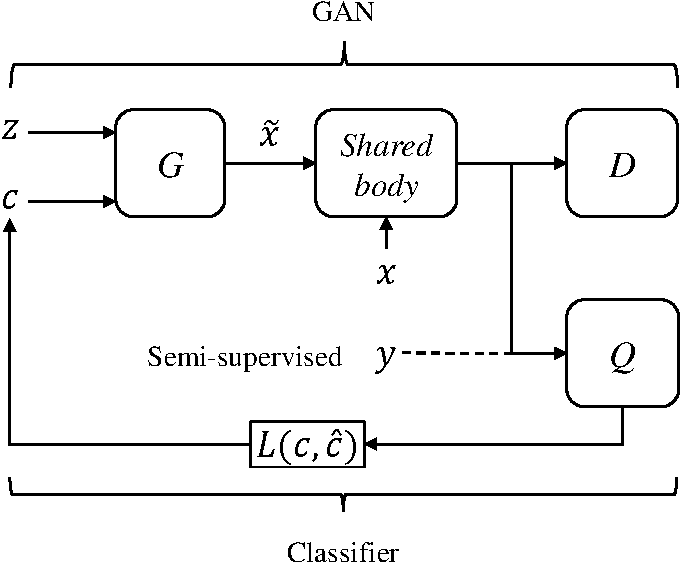
\includegraphics[width=\onef\textwidth]{Img/arch-cinfogan.pdf} 
  \bicaption[C-InfoGAN模型结构示意]
  {C-InfoGAN模型结构。无监督情况下,生成数据$\tilde{\bd{x}}$和真实数据$\bd{x}$参与训练,通过和$D$共享部分结构,$Q$网络可以将GAN模型学习到的特征加以利用,实现分类任务;在半监督情况下,一部分真实标签$y$会直接被$Q$网络利用,以得到更好的效果。模型通过优化$Q$网络的输出$\hat{c}$和隐变量$c$构成的损失函数$L(c,\hat{c})$来增加$Q$的分类准确率。}
  {The architecture of C-InfoGAN. In unsupervised case, the generated data $\tilde{\bd{x}}$ and the real data $\bd{x}$ are used for training. By sharing the body with $D$, $Q$ is able to using features learned by GAN framework to perform classification. In semi-supervised case, labels $y$ is directly fed into $Q$ to get better performance. We optimize the loss function $L(c, \hat{c})$ of latent code $c$ and the output $\hat{c}$ of $Q$ to improve its accuracy.}
  \label{fig:c-infogan}
\end{figure}

使用InfoGAN做分类并不是一个新的想法,\citet{zhang2018cramer}基于InfoGAN提出了一种无监督分类方法。他们生成对抗网络训练的同时,训练一个Parital Inverse Filter (PIF),它接受一个样本作为输入,输出一个和隐变量同维度的向量。之所以叫做PIF,是因为它可以看作生成器$G$的逆映射,将数据映射到隐空间,但又不是完全还原输出噪声,它只输出噪声中的隐变量部分。在训练过程中,他们将PIF的输出与隐变量作均方误差,使得PIF的输出和隐变量的取值尽可能接近。事实上,这个PIF和InfoGAN中的辅助网络具有类似的作用,都是和输入噪声中的隐变量发生联系,而实践发现,使用$Q$网络做分类已经具有可观的效果,而且对计算量的增加较小,模型结构也相对简单。

算法~\ref{alg:cig}给出了C-InfoGAN的训练步骤,其中$\theta_g,~\theta_d,~\theta_q$分别是$G, ~D$和$Q$的网络参数。
\begin{algorithm}[htbp]
  \small
  \caption{Training procedure for C-InfoGAN}
  \label{alg:cig}
  \begin{algorithmic}[1]
    \For{numbers of training iterations}
      \State Sample a batch of $\bd{x} \sim p_{\text{data}}(x)$ of size $m$.
      \State Sample a batch of noise $\bd{z}\sim p_z, ~\bd{c}\sim p_c$ of size
      $m$.
      \State Update the discriminator by ascending its stochastic gradient:
      \[
        \nabla_{\theta_d} \left[ 
          \frac{1}{m} \sum_{i=1}^m \Big( 
            \log D\left(\bd{x}_i\right) + 
            \log\left( 1 - D\left( G(\bd{z}_i, \bd{c}_i) \right) \right)
          \Big)
        \right].
      \]
      \State Update $G$ and $Q$ by descending along its stochastic gradient:
      \[
        \nabla_{\theta_g,\theta_q} \left[ 
          \frac{1}{m} \sum_{\tilde{\bd{x}}} \Big(
            \log(1 - D(G(\bd{z},\bd{c}))) -
            p(\bd{c})\log Q(G(\bd{z}, \bd{c}))
          \Big)
        \right].
      \]
    \EndFor
  \end{algorithmic}
\end{algorithm}


\subsection{半监督分类方法}
%无监督的InfoGAN虽然已经取得非常好的生成效果,但是分类准确率并不是很高。一个自然的想法是通过添加少量标签信息能否使得生成效果更好,分类更准确?答案是肯定的。特别的,
当拥有少量标签信息时,C-InfoGAN可以利用这些标签进一步提升分类准确率和生成效果。同时将隐变量$c$直接绑定到真实的标签,实现精准调控。
%我们可以通过添加少量的标签信息,
%指导隐变量$c$更好地绑定到类别特征,实现精确地调控。
%另外,精确绑定到类别特征的隐变量$c$可以作为直接作为数据的真实标签使用。也就是说,当我们设定$c=1$的时候,生成器就会生成真实类别为`1'的数据。此时,$\argmax_c Q(c|\bd{x})$即可作为分类器的预测值。
针对拥有少量标注信息的情况,\citet{spurr2017guiding}提出半监督的InfoGAN模型,称为ss-InfoGAN。图~\ref{fig:arch-ssinfogan}给出了其模型结构\footnote{ss-InfoGAN模型结构图摘自\citet{spurr2017guiding}。},ss-InfoGAN将隐变量$c$进一步分解为无监督部分$c_{us}$,负责捕捉大量无标注数据的潜在特征;和有监督部分$c_{ss}$,负责捕捉已有标签$y$。同时他们设置了两组隐变量对应的先验分布$P_{c_{us}}$和$P_{c_{ss}}$,以及对应的辅助网络$Q_{us}$和$Q_{ss}$,使用隐变量$c_{ss}$和辅助网络$Q_{ss}$专门处理那部分有标注信息。
\begin{figure}[htbp]
  \centering
  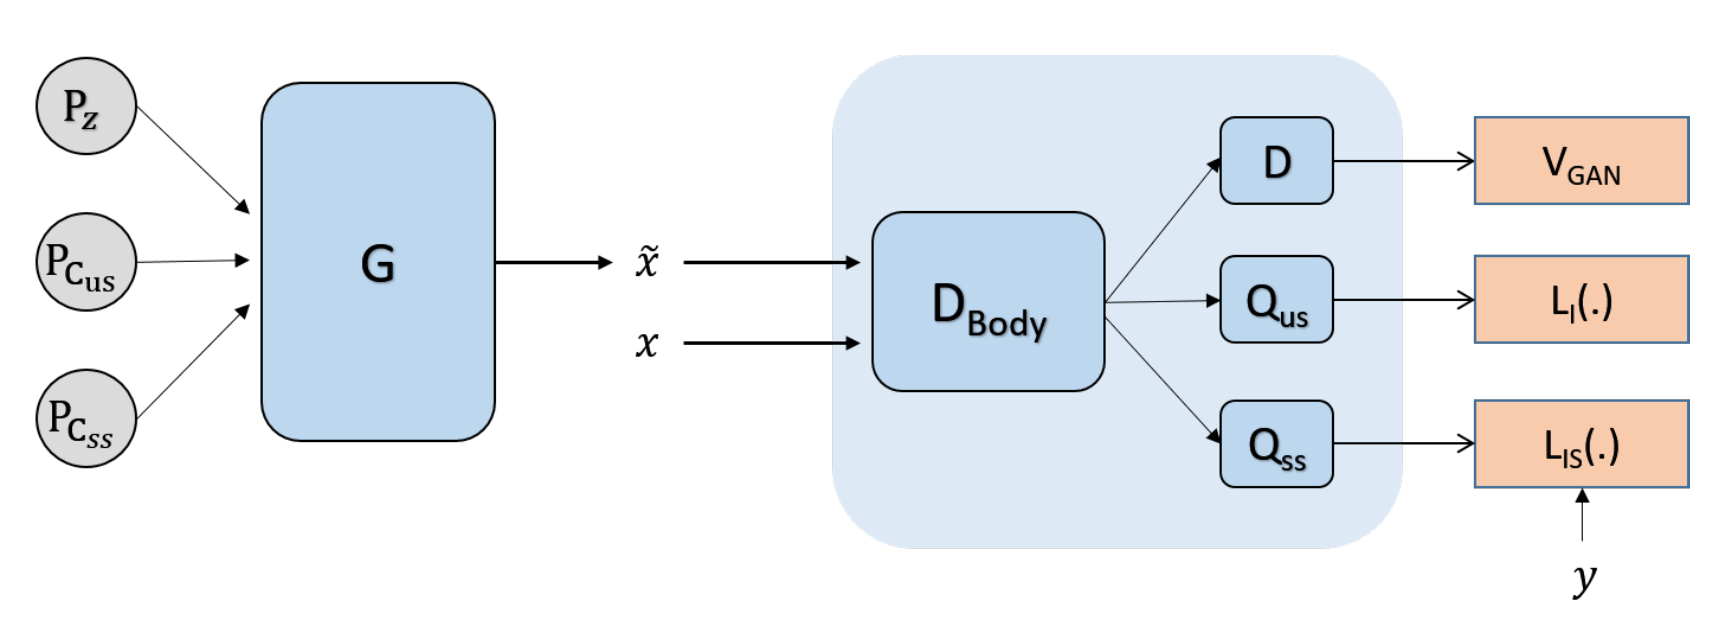
\includegraphics[width=\onef\textwidth]{Img/arch-ssinfogan.png}
  \bicaption{ss-InfoGAN结构示意}{The architecture of ss-InfoGAN}
  \label{fig:arch-ssinfogan}
\end{figure}
本文直接将标签信息加入$Q$网络,先用真实数据和标签训练,接着用生成数据和虚假标签(即隐变量$c$)来训练,这样做的目的是为了使真实标签的信息流入隐变量$c$中,或者可以说是用真实标签指导$c$绑定到正确的类别特征。经过实践发现,简单地使用上述方法也能达到同样的效果,而且模型更为简单。使用和\ref{sec:ss-catgan}节中类似的方法,可以得到半监督C-InfoGAN的目标函数如下:
\begin{equation}\label{eq:ss-cinfogan-obj}
  \begin{split}
  \min_{G,Q}\max_D~ &V_{\text{ss-CIG}}(G,D,Q,\lambda_1,\lambda_2,\lambda_3) = 
  V_{\text{CIG}}(G,D,Q,\lambda_1,\lambda_2) + \\
  &\lambda_3 \E_{(\bd{x}, \bd{y}) \in \Set{L}}
  \left[ \CE[\bd{y}, Q(y|\bd{x})] \right].
  \end{split}
\end{equation}
其中$\lambda_3$为正则化系数,模型结构参见图~\ref{fig:c-infogan}。

算法~\ref{alg:ss-cig}给出了半监督版本的C-InfoGAN的训练步骤,其中$\theta_g, ~\theta_d, ~\theta_g$分别为$G, ~D$和$Q$的网络参数。可以看到,第\ref{ln:bid}行直接将有标签数据放入$Q$网络中训练,通过$Q$网络让标签信息流入虚假标签。在这种情况下,训练稳定之后绑定到类别的隐变量能够和真实标签一一对应(参见~\ref{sec:results}节)。在半监督学习中,如何充分利用有标签数据是一个很重要的问题。在算法~\ref{alg:ss-cig}中,
%做成功概率为$p$的Bernoulli试验。用随机变量$X$表示试验结果,
采用投掷硬币的方式决定如何采样。投掷一枚不公平硬币,正面向上的概率为$p$。设随机变量$X$表示投掷一次该硬币产生的结果,如正面向上,则$X=1$,反之$X=0$,
显然$X\sim\text{Bern}(p)$。
每一次采样前,投掷一次硬币,如果正面向上,则从有标签的数据中采样,否则从无标签数据采样。随着迭代次数的增加,逐渐减小成功概率$p$至某个确定的值。这样做的好处是当$p$减小到最小值之后,虽然由无标签数据占据主导,但还是会偶尔出现一两个有标签的数据批次参与训练,给予无监督训练一定的指导。
\begin{algorithm}[htbp]
  \small
  \caption{Training procedure for semi-supervised C-InfoGAN}
  \label{alg:ss-cig}
  \begin{algorithmic}[1]
    \For{numbers of training iterations}
      \State Sample \texttt{flag} from $\text{Bern}(p)$.
      \Comment{Toss a coin to decide whether to use labels}
      \If{\texttt{flag} is 1}
        \State Sample a batch of labeled samples 
               $(\bd{x}, y) \sim p_{\text{data}}(x,y)$ of size $m$.
      \Else
        \State Sample a batch of unlabeled samples $\bd{x} \sim p_{\text{data}}(x)$ of
        size $m$.
      \EndIf
      \State Sample a batch of noise $\bd{z}\sim p_z, ~\bd{c}\sim p_c$ of size
      $m$.
      \State Update the discriminator by ascending its stochastic gradient:
      \[
        \nabla_{\theta_d} \left[ 
          \frac{1}{m} \sum_{i=1}^m \Big( 
            \log D\left(\bd{x}_i\right) + 
            \log\left( 1 - D\left( G(\bd{z}_i, \bd{c}_i) \right) \right)
          \Big)
        \right].
      \]
      \If{\texttt{flag} is 1}
        \State Update $Q$ by ascending its stochastic gradient: \label{ln:bid}
        \Comment{Bind real labels to fake}
        \[
          \nabla_{\theta_q} \left[ 
            \frac{1}{m} \sum_{(\bd{x}, y)} p(y|\bd{x}) \log Q(\bf{x}) 
          \right].
        \]
      \EndIf
      \State Update $G$ and $Q$ by descending along its stochastic gradient:
      \[
        \nabla_{\theta_g,\theta_q} \left[ 
          \frac{1}{m} \sum_{\tilde{\bd{x}}} \Big(
            \log(1 - D(G(\bd{z},\bd{c}))) -
            p(\bd{c})\log Q(G(\bd{z}, \bd{c}))
          \Big)
        \right]. \label{ln:test}
      \]
      \State $p \gets \max(0.01, \text{Annealing}(p, iterations))$ 
      \Comment{Gradually anneals $p$ to 0.01}
    \EndFor
    %\Procedure{Euclid}{$a,b$}\Comment{The g.c.d. of a and b}
    %\State $r\gets a\bmod b$
    %\While{$r\not=0$}\Comment{We have the answer if r is 0}
    %\State $a\gets b$
    %\State $b\gets r$
    %\State $r\gets a\bmod b$
    %\EndWhile\label{euclidendwhile}
    %\State \textbf{return} $b$\Comment{The gcd is b}
    %\EndProcedure
  \end{algorithmic}
\end{algorithm}

%----------------------------------------------------------------------
\section{InfoCatGAN}\label{sec:icg}
生成对抗网络具有很高的可扩展性,自提出以来应用广泛。\citet{salimans2016improved,odena2016semi}提出使用生成对抗网络模型做半监督分类。在他们的模型中,判别器需要输出$K+1$个类别。考虑一个传统分类模型,给定输入$x$,分类器需要将其分类到$K$个类别中的一个。这样的模型通常接受$x$为输入,输出一个$K$维向量$(\ell_1, \dots, \ell_K)$。通过softmax变换可以将这个向量转化为类别概率$p(y=j|x) = \frac{\exp(\ell_j)}{\sum_{k=1}^K \exp(\ell_k)}$。现考虑使用生成对抗网络做分类,可以通过增加一个类别来对应生成器生成的虚假数据。也就是说,判别器将所有数据分为$K+1$个类别$\Omega = \{\omega_1, \dots, \omega_K, \omega_{K+1}\}$,其中$\omega_{K+1}$对应虚假数据类别。此时,可以用$p(y=\omega_{K+1}|x)$来表示$x$为虚假数据的概率,对应朴素GAN模型中的$1 - D(x)$。对于大量无标签数据,可以通过最大化$\log p(y\in \{\omega_1,\dots,\omega_K\} | x)$来训练分类器。也就是说在给定少量标签的情况下,对于真实数据和虚假数据都有了对应的损失函数
\begin{align}
  L_{\text{ss}} &= -\E_{x,y \sim p_{\text{data}}(x,y)}[\log p(y|x)], \\
  L_{\text{us}} &= -\E_{x\sim p_{\text{data}}(x)}\log [1 - p(y=\omega_{K+1} | x)], \\
  L_{\text{fake}} &= -\E_{x\sim p_g}[\log p(y=\omega_{K+1} | x)],
\end{align}
其中$L_{\text{ss}}, ~L_{\text{us}}, ~L_{\text{fake}}$分别表示针对有标签数据,无标签数据以及虚假数据的损失函数。对于有标签数据,直接利用标签信息优化预测标签和真实标签之间的交叉熵;对于无标签数据,由于标签信息无从得知,所以只能笼统地增加$1-p(y=\omega_{K+1}|x)$来减小被误判的概率;对于虚假数据,都将它判为$\omega_{K+1}$。

\citet{springenberg2015unsupervised}提出的CatGAN模型既可以作无监督分类,也可以做半监督分类。与\citet{salimans2016improved,odena2016semi}类似,CatGAN将判别器扩展为多分类器,令其输出$K$个类别的概率。不同的是,CatGAN重新设计了基于条件熵的损失函数(参见~\ref{sec:catgan})。本节在CatGAN的基础上,添加互信息约束,提出InfoCatGAN模型。该模型同样支持无监督和半监督分类,但是其在生成图片的质量上优于CatGAN。

%\textcolor{red}{improved gan triple gan enhanced triplegan}


\subsection{无监督分类方法}\label{sec:icg-us}
在训练概率分类模型的过程中,通过优化条件熵可以将分类边界调整到更自然的位置(数据分散区域)\cite{grandvalet2005semi},因此CatGAN使用条件熵作为判别器判断真假数据的依据。但是,使用熵作为目标函数的一个缺点是没有类别指向性。考虑一个离散随机变量$Y$表示给定输入$\mathbf{x}$对应的标签,$Y$可能的取值为$\Supp(Y) = \Omega =\{\omega_1, \dots, \omega_K\}$。如果模型仅仅最小化$H(Y|\mathbf{x})$,那么它无法预测$\mathbf{x}$的具体类别。因为任何一个单峰分布都可以使得条件熵达到最小,即$K$个类别中任意一个都可以使$p(y|\mathbf{x})$呈单峰分布,见图~\ref{fig:ent}。
\begin{figure}[htbp]
  \centering
  \begin{subfigure}[b]{\trif\textwidth}
    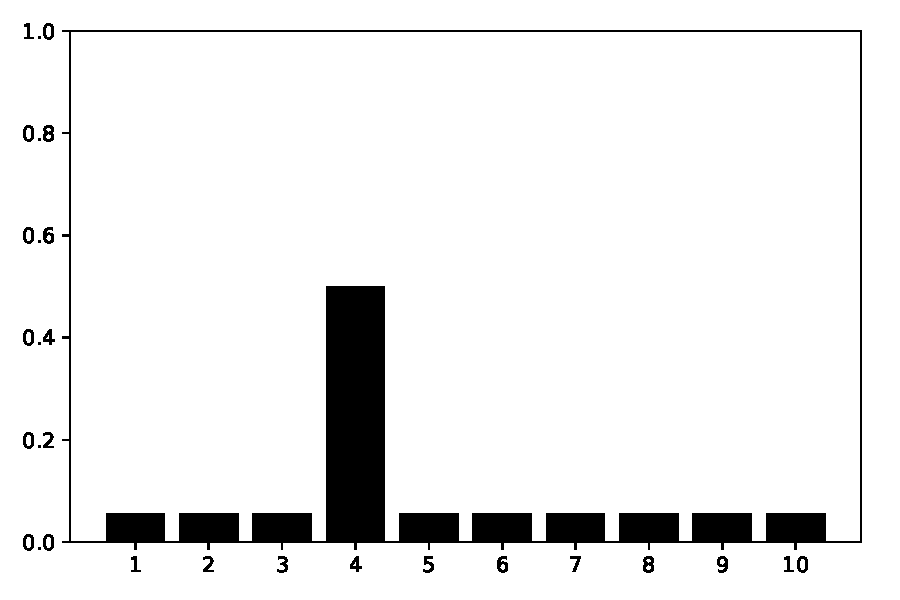
\includegraphics[width=\textwidth]{Img/enta.pdf}
    \caption{$H = 2.58$, predict $y=4$}
  \end{subfigure}
  \begin{subfigure}[b]{\trif\textwidth}
    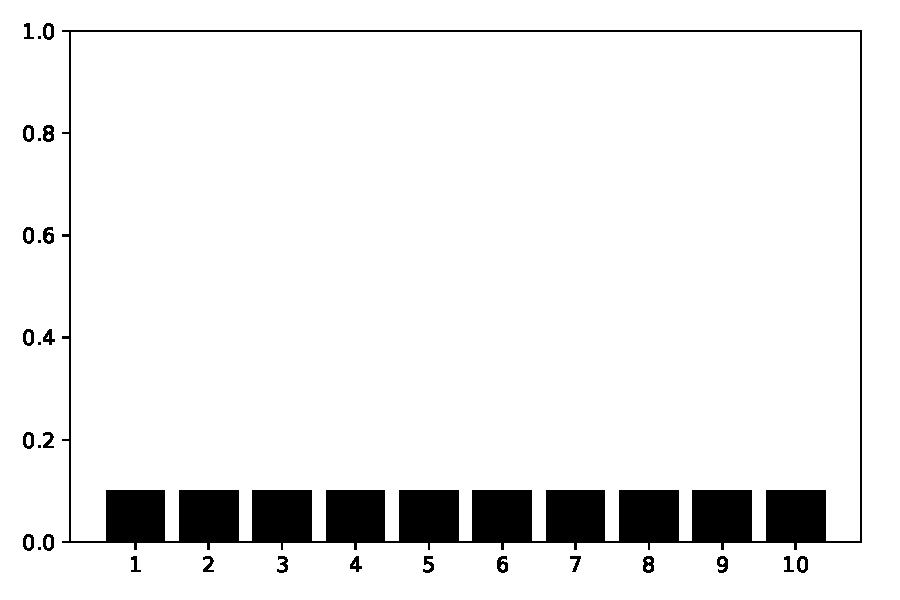
\includegraphics[width=\textwidth]{Img/entb.pdf}
    \caption{$H = 3.32$}
  \end{subfigure}
  \begin{subfigure}[b]{\trif\textwidth}
    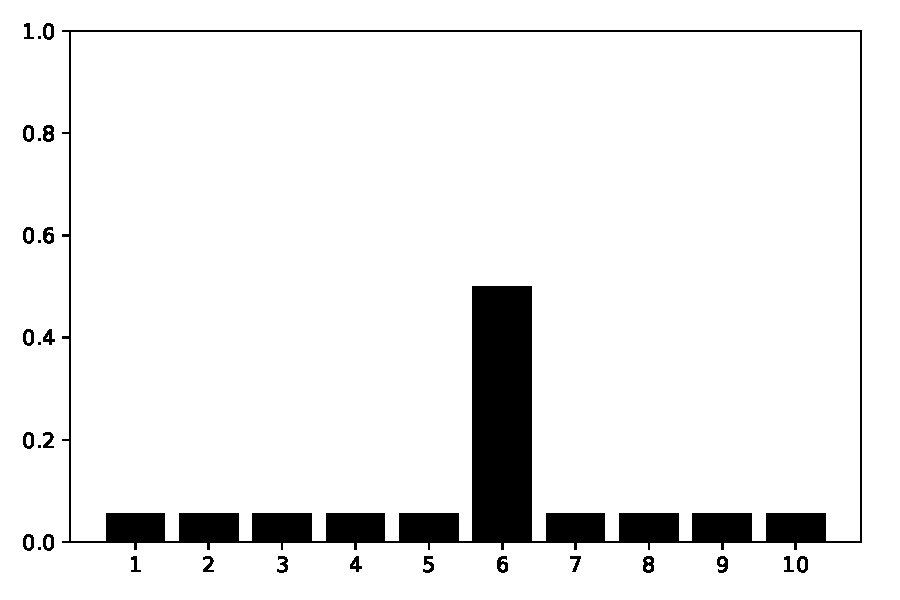
\includegraphics[width=\textwidth]{Img/entc.pdf}
    \caption{$H = 2.58$, predict $y=6$}
  \end{subfigure}
  \bicaption{不同分布的熵}{Entropy of different distributions}
  \label{fig:ent}
\end{figure}
对于分类器而言,希望对于给定输入$\mathbf{x}$,有且仅有一个$k \in [K]$,使得$p(y=\omega_k|\mathbf{x})$最大,而对于任意$k' \neq k, ~p(y=\omega_{k'}|\mathbf{x})$均很小。然而问题在于训练数据集没有标注,每个数据样本对应的标签无从获得。

对于上述问题本文从InfoGAN中获得启发,提出InfoCatGAN模型。InfoGAN将输入噪声划分为$\mathbf{z}$和$\mathbf{c}$,实际上是对隐空间的结构进行了人为划分。一部分提供模型的容量,使得模型具有足够的自由度去学习数据的细节(高度耦合的特征);一部分提供隐变量,用于在学习过程中绑定到数据的显著特征(如:MNIST中的数字类别、笔画粗细、角度)。模型的核心思想如下:通过在隐空间构造一维隐变量$c$,在训练过程中将生成数据的类别标签与之绑定,使得可以通过$c$来控制生成数据的类别。
CatGAN对GAN的扩展主要在于改变了判别器的输出结构:为所有真实数据分配一个类别标签而对于虚假数据则保持一个不确定的状态。类似的,生成器应该致力于生成某个具体类别的数据而不是仅仅生成足够逼真的图片。因此,构造的隐变量实际上充当了虚假图片的标签,它在训练过程中约束着生成器生成指定类别的图片。

\begin{figure}[htbp]
  \centering
  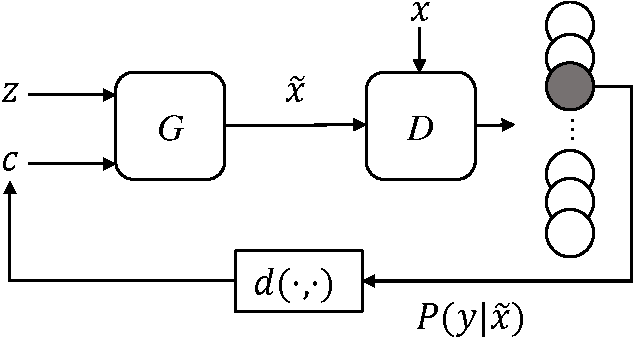
\includegraphics[width=\onef\textwidth]{Img/icg-arch.pdf} 
  \bicaption[InfoCatGAN结构示意]
  {InfoCatGAN模型结构。图中$D$的输出为$P(y|\cdot)$。在训练生成器的时候,将判别器的输出$P(y|\tilde{\mathbf{x}})$和隐变量$c$通过某种度量$d(\cdot, \cdot)$建立联系使得条件概率的峰值与$c$的取值对应。}
  {The architecture of InfoCatGAN. The discriminator outputs $P(y|\cdot)$. When training generator, we add a regularizer $d(\cdot,\cdot)$ between the ouput of discriminator and the latent code $c$ to match the peak of $P(y|\tilde{\mathbf{x}})$ with $c$.}
  \label{fig:icg-arch}
\end{figure}

下面给出InfoCatGAN的损失函数:设$\mathbf{x} \in \mathcal{X}$为一个真实数据样本,$\tilde{\mathbf{x}} = G(\mathbf{z}, c)$为一个生成数据,其中$z\sim p_z$为噪声,$c\sim p_c$为隐变量。为了简单起见,这里只考虑$c$为一维离散随机变量,$p_c$为离散均匀分布。生成器$G = G(\mathbf{z}, c; ~\theta_G)$和判别器$D = D(\mathbf{x}; ~\theta_D)$均为可微深度神经网络,其中$\theta_G, ~\theta_D$分别为生成器和判别器的参数\footnote{参数通常省略。}。通过在$D$网络的最后一层做softmax变换,可以直接将$D(x)$作为条件概率$p(y|x)$的估计。注意到\eqref{eq:catgan-obj}式可以重写为:
\begin{align}
  L_D^{\text{cat}} &= -I(X;Y)-
         \E_{\tilde{\mathbf{x}} \sim p_g}[H(p(y|\tilde{\mathbf{x}}))], \label{eq:lcatd} \\
  L_G^{\text{cat}} &= -I(\tilde{X}; Y), \label{eq:lcatg}
\end{align}
%%NOTE%%
% May have interaction with information bottleneck!
其中$X \sim p_{\text{data}}, ~\tilde{X} \sim p_g$分别表示真实数据和虚假数据对应的随机变量,$Y$表示未知标签对应的随机变量。从\eqref{eq:lcatd}、\eqref{eq:lcatg}式可以看出,CatGAN在优化数据与标签之间的互信息。互信息是常用的变量间相关性的衡量标准,所以本文用它作为生成器损失函数的正则项,由此得到InfoCatGAN的损失函数如下:
\begin{equation}
\label{eq:infocatgan}
\begin{split}
  L_D &= L_D^{\text{cat}}, \\ 
  L_G &= L_G^{\text{cat}} - \lambda_1 I(c; \tilde{\mathbf{x}}),
\end{split}
\end{equation}
其中$\lambda_1$为正则系数,可知当$\lambda_1 = 0$时,InfoCatGAN退化为CatGAN,模型结构见图~\ref{fig:icg-arch}。参考\eqref{eq:infogan-obj}式,$I(c; \tilde{\mathbf{x}})$可以放缩为$\E_{p(\mathbf{c},\tilde{\mathbf{x}})}[\log p(c|\tilde{\mathbf{x}})]$,在实现中通常使用交叉熵
\begin{equation}
  CE[\mathbf{c}, p(c|\tilde{\mathbf{x}})] = -\sum_{i=1}^K c_i \log p(c=c_i | \tilde{\mathbf{x}})
\end{equation}
来优化此项,这里的$\mathbf{c} \in \reals^K$是隐变量$c$经过one-hot编码之后的向量,$p(c|\tilde{\mathbf{x}})$可以用$D(\tilde{\mathbf{x}})$来近似。

算法~\ref{alg:icg}给出了InfoCatGAN的训练步骤,其中$\theta_g,~\theta_d$分别为$G, ~D$的网络参数。第\ref{ln:catd}、\ref{ln:catg}行的更新公式可以参考\eqref{eq:infocatgan}式和\eqref{eq:catgan-obj}式。从第~\ref{ln:catg}行可以看出,算法在训练过程中将隐变量有意识地和虚假图片的类别绑定,这样做的效果是训练稳定后,可以通过隐变量控制生成图片的类别。注意到第\ref{ln:catd}、\ref{ln:catg}行的最后一项分别对应着\eqref{eq:catgan-obj}中的$H_{\Set{X}}(p(y))$和$H_{G}(p(y))$,\citet{springenberg2015unsupervised}指出边缘分布的熵的估计方法应当视情况而定。原本$H_{\Set{X}}$应当针对整个训练数据集来计算边缘分布,然后在计算熵;而$H_G$也不能单单只用一个批次的虚假样本计算,应当生成远大于批处理大小的虚假样本来计算边缘分布,再计算熵。但是在批处理大小$m$远大于类别总数$K$(比如$K=10, ~m=100$)的时候,算法~\ref{alg:icg}中对于边缘分布的熵的估计是合理的\footnote{本文在实验中也采用了校正后的边缘分布的熵的估计方法,发现这对实验结果影响并不大。}。
\begin{algorithm}[htbp]
  \small
  \caption{Training procedure for InfoCatGAN}
  \label{alg:icg}
  \begin{algorithmic}[1]
    \For{numbers of training iterations}
      \State Sample a batch of $\bd{x} \sim p_{\text{data}}(x)$ of size $m$.
      \State Sample a batch of noise $\bd{z}\sim p_z, ~\bd{c}\sim p_c$ of size
      $m$.
      \State Update the discriminator by ascending its stochastic gradient:
      \label{ln:catd}
      \[
        \nabla_{\theta_d} \left[ 
          \frac{1}{m} \sum_{i=1}^m \Big( 
            - H(D(\bd{x}_i)) + H(D(G(\bd{z}_i, \bd{c}_i)))
          \Big) + H\left( \frac{1}{m}\sum_{i=1}^m D(\bd{x}_i) \right)
        \right].
      \]
      \State Update $G$ and $D$ by descending along its stochastic gradient:
      \label{ln:catg}
      \[
        \nabla_{\theta_g,\theta_d} \left[ 
          \frac{1}{m} \sum_{\tilde{\bd{x}} = G(\bd{z},\bd{c})} \Big(
            H(D(\tilde{\bd{x}})) - p(\bd{c})\log D(\tilde{\bd{x}})
          \Big)
          - H \left( 
            \frac{1}{m}\sum_{i=1}^m D(G(\bd{z}_i, \bd{c}_i))
          \right)
        \right].
      \]
    \EndFor
  \end{algorithmic}
\end{algorithm}


\subsection{半监督分类方法}\label{sec:ss-infocatgan}
%%%------> \textcolor{red}{目标写两页}
作为CatGAN的扩展,InfoCatGAN能够很自然地适用于半监督的情况。假设$\Set{L} = \{\mathbf{x}_i, y_i\}_{i=1}^m$为$m$个有标签的样本,$\mathbf{y}_i \in \reals^K$表示标签$y_i$经过one-hot编码之后的向量:即如果$\mathbf{x}_i$的标签是$\omega_k$,则$\mathbf{y}_{ik}=1$且对于所有的$j\neq k,~\mathbf{y}_{ij} = 0$。对于有标签的样本,$D(\mathbf{x})$的分布信息可以明确获得,所以可以通过计算$\mathbf{y}$和$p(y|\mathbf{x})$之间的交叉熵:
\begin{equation}
  \label{eq:celoss}
  \CE[\mathbf{y}, p(y|\mathbf{x})] = -\sum_{i=1}^K y_i \log p(y=y_i | \mathbf{x})
\end{equation}
来辅助判别器做出更精确的判断。半监督版本的InfoCatGAN损失函数如下:
\begin{equation}
  \label{eq:ss-infocatgan-obj}
  L_D^L = L_D + \lambda_2 \E_{(\mathbf{x}, \mathbf{y}) \in \Set{L}}\left[ CE[\mathbf{y}, p(y|\mathbf{x})] \right],
\end{equation}
其中$\lambda_2$为正则系数而生成器的损失函数同\eqref{eq:infocatgan}式:$L_G^L = L_G$.

\begin{algorithm}[htbp]
  \small
  \caption{Training procedure for semi-supervised InfoCatGAN}
  \label{alg:ss-icg}
  \begin{algorithmic}[1]
    \For{numbers of training iterations}
      \State Sample \texttt{flag} from Bern($p$).
      \If{\texttt{flag} is 1}
        \State Sample a batch of labeled samples 
        $(\bd{x}, y) \sim p_{\text{data}}(x,y)$ of size $m$.
      \Else
        \State Sample a batch of unlabeled samples 
        $\bd{x} \sim p_{\text{data}}(x)$ of size $m$.
      \EndIf
      \State Sample a batch of noise $\bd{z}\sim p_z, ~\bd{c}\sim p_c$ of size
      $m$.
      \State Update the discriminator by ascending its stochastic gradient:
      \label{ln:catdss}
      \[
        \nabla_{\theta_d} \left[ 
          \frac{1}{m} \sum_{i=1}^m \Big( 
            - H(D(\bd{x}_i)) + H(D(G(\bd{z}_i, \bd{c}_i)))
          \Big) + H\left( \frac{1}{m}\sum_{i=1}^m D(\bd{x}_i) \right)
        \right].
      \]
      \If{\texttt{flag} is 1}
        \State Update $D$ by ascending its stochastic gradient:
        \label{ln:bidd}
        \[
          \nabla_{\theta_d} \left[ 
            \frac{1}{m} \sum_{(\bd{x}, y)} p(y|\bd{x}) \log D(\bf{x}) 
          \right].
        \]
      \EndIf
      \State Update $G$ and $D$ by descending along its stochastic gradient:
      \label{ln:catgss}
      \[
        \nabla_{\theta_g,\theta_d} \left[ 
          \frac{1}{m} \sum_{\tilde{\bd{x}} = G(\bd{z},\bd{c})} \Big(
            H(D(\tilde{\bd{x}})) - p(\bd{c})\log D(\tilde{\bd{x}})
          \Big)
          - H \left( 
            \frac{1}{m}\sum_{i=1}^m D(G(\bd{z}_i, \bd{c}_i))
          \right)
        \right].
      \]
      \State $p \gets \max(0.01, \text{Annealing}(p, iterations))$ 
    \EndFor
  \end{algorithmic}
\end{algorithm}
算法~\ref{alg:ss-icg}给出了半监督版本的InfoCatGAN的训练步骤,其中$\theta_q,~\theta_d$分别为$G,~D$的网络参数。从第\ref{ln:bidd}行可以看出,如果当前批次是有标签的数据,则直接最小化真实标签和预测概率之间的交叉熵。这样做的目的是通过判别器$D$将真实标签信息流入虚假标签,即隐变量中。训练稳定之后,虚假标签和真实标签会一一对应(参见~\ref{sec:results}节)。在半监督版本的训练中,首先将数据集分为有标签部分和无标签部分,这里同样采用投掷硬币的方式,决定从哪个数据集采样。

\section{本章小结}
本章首先介绍了生成对抗网络的可扩展性:可以添加条件信息学习条件分布;可以增加逆向网络,通过数据空间推断隐空间;可以加入少量标签与半监督学习结合。接着介绍了本文提出的两个模型:C-InfoGAN和InfoCatGAN,这两个模型都可以做到无监督和半监督的分类,并且都利用了互信息约束。第一节详细阐述了无监督和半监督C-InfoGAN的模型结构及理论,并给出了具体的训练算法。第二节详细阐述了无监督和半监督InfoCatGAN的模型结构及理论,并给出了相应的训练算法。具体的实现细节和实验结果将在第\ref{chap:experiments}章给出。
